%fich.tex
%%%%%%%%%%%%%%%%%%%%%%%%%%%%%%%%%%%%%%%%%%%%%%%%%%%%%%%%%%%%%%%%%%%%%%%%
% Fco. Javier Bóhorquez Ogalla
% Descripción del documento:
	
%%%%%%%%%%%%%%%%%%%%%%%%%%%%%%%%%%%%%%%%%%%%%%%%%%%%%%%%%%%%%%%%%%%%%%%%


%%%%%%%%%%%%%%%%%%%%%%%%%%%%%%%%%%%%%%%%%%%%%%%%%%%%%%%%%%%%%%%%%%%%%%%%
%Clase de documento
\documentclass[12pt, spanish]{article}
%%%%%%%%%%%%%%%%%%%%%%%%%%%%%%%%%%%%%%%%%%%%%%%%%%%%%%%%%%%%%%%%%%%%%%%%


%%%%%%%%%%%%%%%%%%%%%%%%%%%%%%%%%%%%%%%%%%%%%%%%%%%%%%%%%%%%%%%%%%%%%%%%	
%Paquetes de lenguaje:
%%%%%%%%%%%%%%%%%%%%%%%%%%%%%%%%%%%%%%%%%%%%%%%%%%%%%%%%%%%%%%%%%%%%%%%%
\usepackage[utf8]{inputenc}
\usepackage[spanish]{babel}
%\usepackage[spanish, activeacute] {babel}	
%\usepackage[spanish]{babel} 				
%\usepackage[latin1]{inputenc}
%%%%%%%%%%%%%%%%%%%%%%%%%%%%%%%%%%%%%%%%%%%%%%%%%%%%%%%%%%%%%%%%%%%%%%%%

%%%%%%%%%%%%%%%%%%%%%%%%%%%%%%%%%%%%%%%%%%%%%%%%%%%%%%%%%%%%%%%%%%%%%%%%
%Gramatic

\usepackage{/usr/share/texlive/texmf-dist/tex/latex/base/bnf}
%%%%%%%%%%%%%%%%%%%%%%%%%%%%%%%%%%%%%%%%%%%%%%%%%%%%%%%%%%%%%%%%%%%%%%%%

%%%%%%%%%%%%%%%%%%%%%%%%%%%%%%%%%%%%%%%%%%%%%%%%%%%%%%%%%%%%%%%%%%%%%%%%
%Paquetes para encabezados y pie de páginas
%%%%%%%%%%%%%%%%%%%%%%%%%%%%%%%%%%%%%%%%%%%%%%%%%%%%%%%%%%%%%%%%%%%%%%%%
\usepackage{fancyhdr}
%%%%%%%%%
% \pagestyle{fancy} %Si se cambia el estilo de página, antes de empezar 
	%el documento. Esto hace que el emcabezado y pie de página se 
	%quede separado del texto por una línea
%%%%%%%%%	
% \fancyhead{} % Límpia el texto que se está usando como encabezado
%%%%%%%%%
% \fancyhead[OPCIONES]{Encabezado}
	% OPCIONES:
		% L texto a la izquierda
		% C texto centrado
		% R texto a la derecha
		% E página par
		% O pagina impar
	%Ejemplo: 
		% fancyhead [LE] {"Doc. Latex"} 
			% Establece como emcabezado de las páginas pares "Doc Latex"
			% con alineacion a la izquierda
%%%%%%%%%			
% \fancyfoot[OPCIONES]{Píe de pag.}
	% OPCIONES:
		% L C R E O
	%Ejemplo
		% \fancyfoot[LE,RO]{\thepage} 
			% Establece como píe de pág. el número de página. con 
			% alineación a la izq en paginas pares y a la derecha en
			% las impares
%%%%%%%%%			
% \renewcommand{\headrulewidth}{0.4pt}
% \renewcommand{\footrulewidth}{0.4pt}
	% Fija el grosor de la la linea que separa el emcabezado y pie de pág
%%%%%%%%%
% Otros comandos:
%\lhead{}
%\chead{}
%\rhead{}
%\lfoot{}
%\cfoot{}
%%%%%%%%%%%%%%%%%%%%%%%%%%%%%%%%%%%%%%%%%%%%%%%%%%%%%%%%%%%%%%%%%%%%%%%%


%%%%%%%%%%%%%%%%%%%%%%%%%%%%%%%%%%%%%%%%%%%%%%%%%%%%%%%%%%%%%%%%%%%%%%%%
% Paquetes para tamaños y distancias
%%%%%%%%%%%%%%%%%%%%%%%%%%%%%%%%%%%%%%%%%%%%%%%%%%%%%%%%%%%%%%%%%%%%%%%%
\usepackage{anysize} 
%%%%%%%%%%%
% \marginsize{3cm}{2cm}{2cm}{2cm}
	% Controla los márgenes {izquierda}{derecha}{arriba}{abajo}. 
%%%%%%%%%%%%%%%%%%%%%%%%%%%%%%%%%%%%%%%%%%%%%%%%%%%%%%%%%%%%%%%%%%%%%%%%


%%%%%%%%%%%%%%%%%%%%%%%%%%%%%%%%%%%%%%%%%%%%%%%%%%%%%%%%%%%%%%%%%%%%%%%%
%Paquetes de carácteres especiales:
%%%%%%%%%%%%%%%%%%%%%%%%%%%%%%%%%%%%%%%%%%%%%%%%%%%%%%%%%%%%%%%%%%%%%%%%
\usepackage{dsfont}	
%Para representar conjuntos matematicos comunes: Z, N, R...
	% mathds{R}, mathds{N},...
%%%%%%%%%%%%%%%%%%%%%%%%%%%%%%%%%%%%%%%%%%%%%%%%%%%%%%%%%%%%%%%%%%%%%%%%

%%%%%%%%%%%%%%%%%%%%%%%%%%%%%%%%%%%%%%%%%%%%%%%%%%%%%%%%%%%%%%%%%%%%%%%%
%Paquetes para insertar gráficos
%%%%%%%%%%%%%%%%%%%%%%%%%%%%%%%%%%%%%%%%%%%%%%%%%%%%%%%%%%%%%%%%%%%%%%%%
\usepackage[dvips]{graphicx}
\DeclareGraphicsExtensions{.pdf,.png,.jpg} %solo para PDFLaTeX
%%%%%%%%%%%%%%%%%%%%%%%%%%%%%%%%%%%%%%%%%%%%%%%%%%%%%%%%%%%%%%%%%%%%%%%%

%%%%%%%%%%%%%%%%%%%%%%%%%%%%%%%%%%%%%%%%%%%%%%%%%%%%%%%%%%%%%%%%%%%%%%%%
%Paquetes de color:
%%%%%%%%%%%%%%%%%%%%%%%%%%%%%%%%%%%%%%%%%%%%%%%%%%%%%%%%%%%%%%%%%%%%%%%%
\usepackage{color}
%%%%%%%%%%%%%%%%%%%%%%%%%%%%%%%%%%%%%%%%%%%%%%%%%%%%%%%%%%%%%%%%%%%%%%%%
%Definición de colores:
\definecolor{gray97}{gray}{.97}
\definecolor{gray75}{gray}{.75}
\definecolor{gray45}{gray}{.45}
%%%%%%%%%%%%%%%%%%%%%%%%%%%%%%%%%%%%%%%%%%%%%%%%%%%%%%%%%%%%%%%%%%%%%%%%
\usepackage{multicol}

%%%%%%%%%%%%%%%%%%%%%%%%%%%%%%%%%%%%%%%%%%%%%%%%%%%%%%%%%%%%%%%%%%%%%%%%
%Paquete de listado de código:
%%%%%%%%%%%%%%%%%%%%%%%%%%%%%%%%%%%%%%%%%%%%%%%%%%%%%%%%%%%%%%%%%%%%%%%%
\usepackage{listings}
%%%%%%%%%%%%%%%%%%%%%%%%%%%%%%%%%%%%%%%%%%%%%%%%%%%%%%%%%%%%%%%%%%%%%%%%
%Configuración del listado:

\lstset { 
	frame=Ltb,
     framerule=0pt,
     aboveskip=0.2cm,
     framextopmargin=0.3pt,
     framexbottommargin=0.2pt,
     framexleftmargin=0.3cm,
     framesep=0pt,
     rulesep=.1pt,
     tabsize=2,
     backgroundcolor=\color{gray97},
     rulesepcolor=\color{black},
     %
     stringstyle=\ttfamily,
     showstringspaces = false,
     basicstyle=\scriptsize\ttfamily,
     commentstyle=\color{gray45},
     keywordstyle=\bfseries,
   	%
     numbers=left,
     numbersep=1pt,
     numberstyle=\tiny,
     numberfirstline = false,
     breaklines=true,
}
%%%%%%%%%%%%%%%%%%%%%%%%%%%%%%%%%%%%%%%%%%%%%%%%%%%%%%%%%%%%%%%%%%%%%%%%


%%%%%%%%%%%%%%%%%%%%%%%%%%%%%%%%%%%%%%%%%%%%%%%%%%%%%%%%%%%%%%%%%%%%%%%%
%Indexado. Índice alfabeticos
\usepackage{makeidx}
\makeindex %para habilitar indices
%%%%%%%%%%%%%%%%%%%%%%%%%%%%%%%%%%%%%%%%%%%%%%%%%%%%%%%%%%%%%%%%%%%%%%%%
%Forma de uso:
% \index{clave} %Para crear un indice de materia
% Supongase que queremos meter en el indice alfabetico referencias a 
% las paginas donde se hace referencia a la clave Producto escalar
% en tal caso en cada una de las páginas pondremos \index{Producto escalar}
% \printindex %Para imprimir el índice alfabetico

% Es necesario una doble compilación del documento. La primera genera un 
% fichero.idx el cual tendremos que procesar con la aplicación makeindex
%tras procesarlo se creará un fichero.ind que contendra el código Latex 
% que se inserta en el documento original. 
% Tras la segunda compilación del documento original se sustituira el
% comando \printindex por el contenido del fichero.ind 

%Podemos cambiar el formato de la clave:
%Ejemplo     				&    	Entrada 		&	Comentario
%\index{hola}				&         hola, 1   	&	Entrada simple
%\index{hola!Pedro}			&		 Pedro, 3 	&	Subentrada bajo ‘hola’
%\index{Juan@\textsl{Juan}}  	&		Juan, 2    	&	Entrada con diseño                        
%\index{Pepa@\textbf{Pepa}}	&		Pepa, 7    	&	Igual que antes
%\index{Loli|textbf}		&		Loli, 3    	&	No de página con diseño                     
%\index{Soraya|textit}		&		Soraya, 5  	&	Igual que antes
%%%%%%%%%%%%%%%%%%%%%%%%%%%%%%%%%%%%%%%%%%%%%%%%%%%%%%%%%%%%%%%%%%%%%%%%


%%%%%%%%%%%%%%%%%%%%%%%%%%%%%%%%%%%%%%%%%%%%%%%%%%%%%%%%%%%%%%%%%%%%%%%%


%%%%%%%%%%%%%%%%%%%%%%%%%%%%%%%%%%%%%%%%%%%%%%%%%%%%%%%%%%%%%%%%%%%%%%%%
%Estilo de página
%%%%%%%%%%%%%%%%%%%%%%%%%%%%%%%%%%%%%%%%%%%%%%%%%%%%%%%%%%%%%%%%%%%%%%%%
%\textwidth 6.75in								  %ancho de texto
%\oddsidemargin -0.2in							%margen izquierdo 
\parskip 0.2in									%espacio parrafos
%%%%%%%%%%%%%%%%%%%%%%%%%%%%%%%%%%%%%%%%%%%%%%%%%%%%%%%%%%%%%%%%%%%%%%%%
\newenvironment{changemargin}[2]{%
\begin{list}{}{%
\setlength{\topsep}{300pt}%
\setlength{\leftmargin}{#1}%
\setlength{\rightmargin}{#2}%
\setlength{\listparindent}{\parindent}%
\setlength{\itemindent}{\parindent}%
\setlength{\parsep}{\parskip}%
}%
\item[]}{\end{list}}
%%%%%%%%%%%%%%%%%%%%%%%%%%%%%%%%%%%%%%%%%%%%%%%%%%%%%%%%%%%%%%%%%%%%%%%%
\usepackage{float}
\restylefloat{table}
\usepackage{placeins}
\usepackage{framed}
\usepackage{epsf}
%%%%%%%%%%%%%%%%%%%%%%%%%%%%%%%%%%%%%%%%%%%%%%%%%%%%%%%%%%%%%%%%%%%%%%%%

\usepackage{titlesec}

\setcounter{secnumdepth}{4}

\titleformat{\paragraph}
{\normalfont\normalsize\bfseries}{\theparagraph}{1em}{}
\titlespacing*{\paragraph}
{0pt}{3.25ex plus 1ex minus .2ex}{1.5ex plus .2ex}


%%%%%%%%%%%%%%%%%%%%%%%%%%%%%%%%%%%%%%%%%%%%%%%%%%%%%%%%%%%%%%%%%%%%%%%%	
%datos del documento
\author{Construcción del sistema \\\\\ Fco. Javier Bohórquez Ogalla}						%autor
\date{}														%fecha

\title{ 
\begin{center}

\includegraphics[scale=0.5]{logo-doc.png}
\end{center} 
}
%%%%%%%%%%%%%%%%%%%%%%%%%%%%%%%%%%%%%%%%%%%%%%%%%%%%%%%%%%%%%%%%%%%%%%%%

%%%%%%%%%%%%%%%%%%%%%%%%%%%%%%%%%%%%%%%%%%%%%%%%%%%%%%%%%%%%%%%%%%%%%%%%
%Documento:
%%%%%%%%%%%%%%%%%%%%%%%%%%%%%%%%%%%%%%%%%%%%%%%%%%%%%%%%%%%%%%%%%%%%%%%%
\lstdefinestyle{nonumbers}{numbers=none}
\begin{document}

\maketitle
\pagebreak
\tableofcontents
\pagebreak
\section{Vista general}
En esta sección se tratan los aspectos relacionados con la con la implementación
del sistema y su codificación. Para ello se describen las herramientas software
y hardware utilizadas en el desarrollo, y la estructra del código fuente. 

\section{Entorno de construcción}

\begin{description}
   \item[Entodrno de desarrollo (IDE):] Geany
   \item[Lenguaje de programación:] C++
   \item[Compilador:] GCC
   \item[Configuración automática:] Autoconf
   \item[Construcción automática:] Automake
   \item[Gestión de dependencias:] Make
   \item[Control de versions:] Subversion
   \item[Generador de analizador léxico:] Flex
   \item[Generador de analizador sintáctico:] Bison
   \item[Depurador:] GDB
   \item[Bibliotecas de desarrollo] \hfill 
      \begin{description}
         \item[Editor de línea e histórico:] Readline
         \item[Expresiones regulares:] BoostRegex
         \item[Matemáticas:] Biblioteca estándar de C
         \item[Enlaces dinámicos:] Biblioteca del sistema GNU/Linux libdl
      \end{description}
   \item[Desarrollo Web] \hfill 
      \begin{description}
         \item[Programación en servidor:] PHP
         \item[Programación en cliente:] JavaScript
         \item[Estructura del contenido:] HTML5
         \item[Presentación del contenido:] CSS
      \end{description}
\end{description}

\section{Ficheros de código fuente}
El sistema software se constituye de una serie de módulos o componentes en forma de ficheros, 
cada uno de los cuales contiene las estructuras de programación y el código fuente necesario
para implementar cada una de las funcionalidades del sistema.

\begin{description}
\item [interpreter:] Interprete.
\item [lshScanner:] Analizador léxico.
\item [lshParser:] Analizador sintáctico.
\item [error:] Sistema de errores.
\item [plugins:] Sistema de extensiones.
\item [run/runTree:] Abstracción de nodo ejecutable.
\item [run/expNode:] Abstracción de nodos ejecutables expresiones.
\item [run/symbols:] Estructura de datos tabla de símbolos.
\item [run/sTable:] Gestión de tabla de de símbolos y definiciones.
\item [run/typeNode:] Nodos ejecutables para cada tipo de dato.
\item [run/numData:] Representación interna de datos numéricos.
\item [run/stmtNode:] Nodos ejecutables sentencias de control.
\item [run/operatorBaseNode:] Nodos ejecutables operadores básicos.
\item [run/operatorLogicNode:] Nodos ejecutables operadores lógicos.
\item [run/operatorArithNode:] Nodos ejecutables operadores aritméticos.
\item [run/operatorStrNode:] Nodos ejecutables operadores sobre cadenas.
\item [run/operatorArrayNode:] Nodos ejecutables operadores sobre arrays.
\item [run/operatorRegexpNode:] Nodos ejecutables operadores sobre expresiones regulares.
\item [run/operatorDateNode:] Nodos ejecutables operadores sobre fechas y tiempo.
\item [run/operatorFileNode:] Nodos ejecutables operadores sobre ficheros.
\item [run/operatorProcessNode:] Nodos ejecutables operadores sobre procesos.
\end{description}

A continuación se describen las dependencias entre ficheros mediante una serie de paquetes que contienen diagramas de componentes.
Este aspecto del sistema queda completamente descrito mediante la combinación de estos paquetes.

\begin{center}
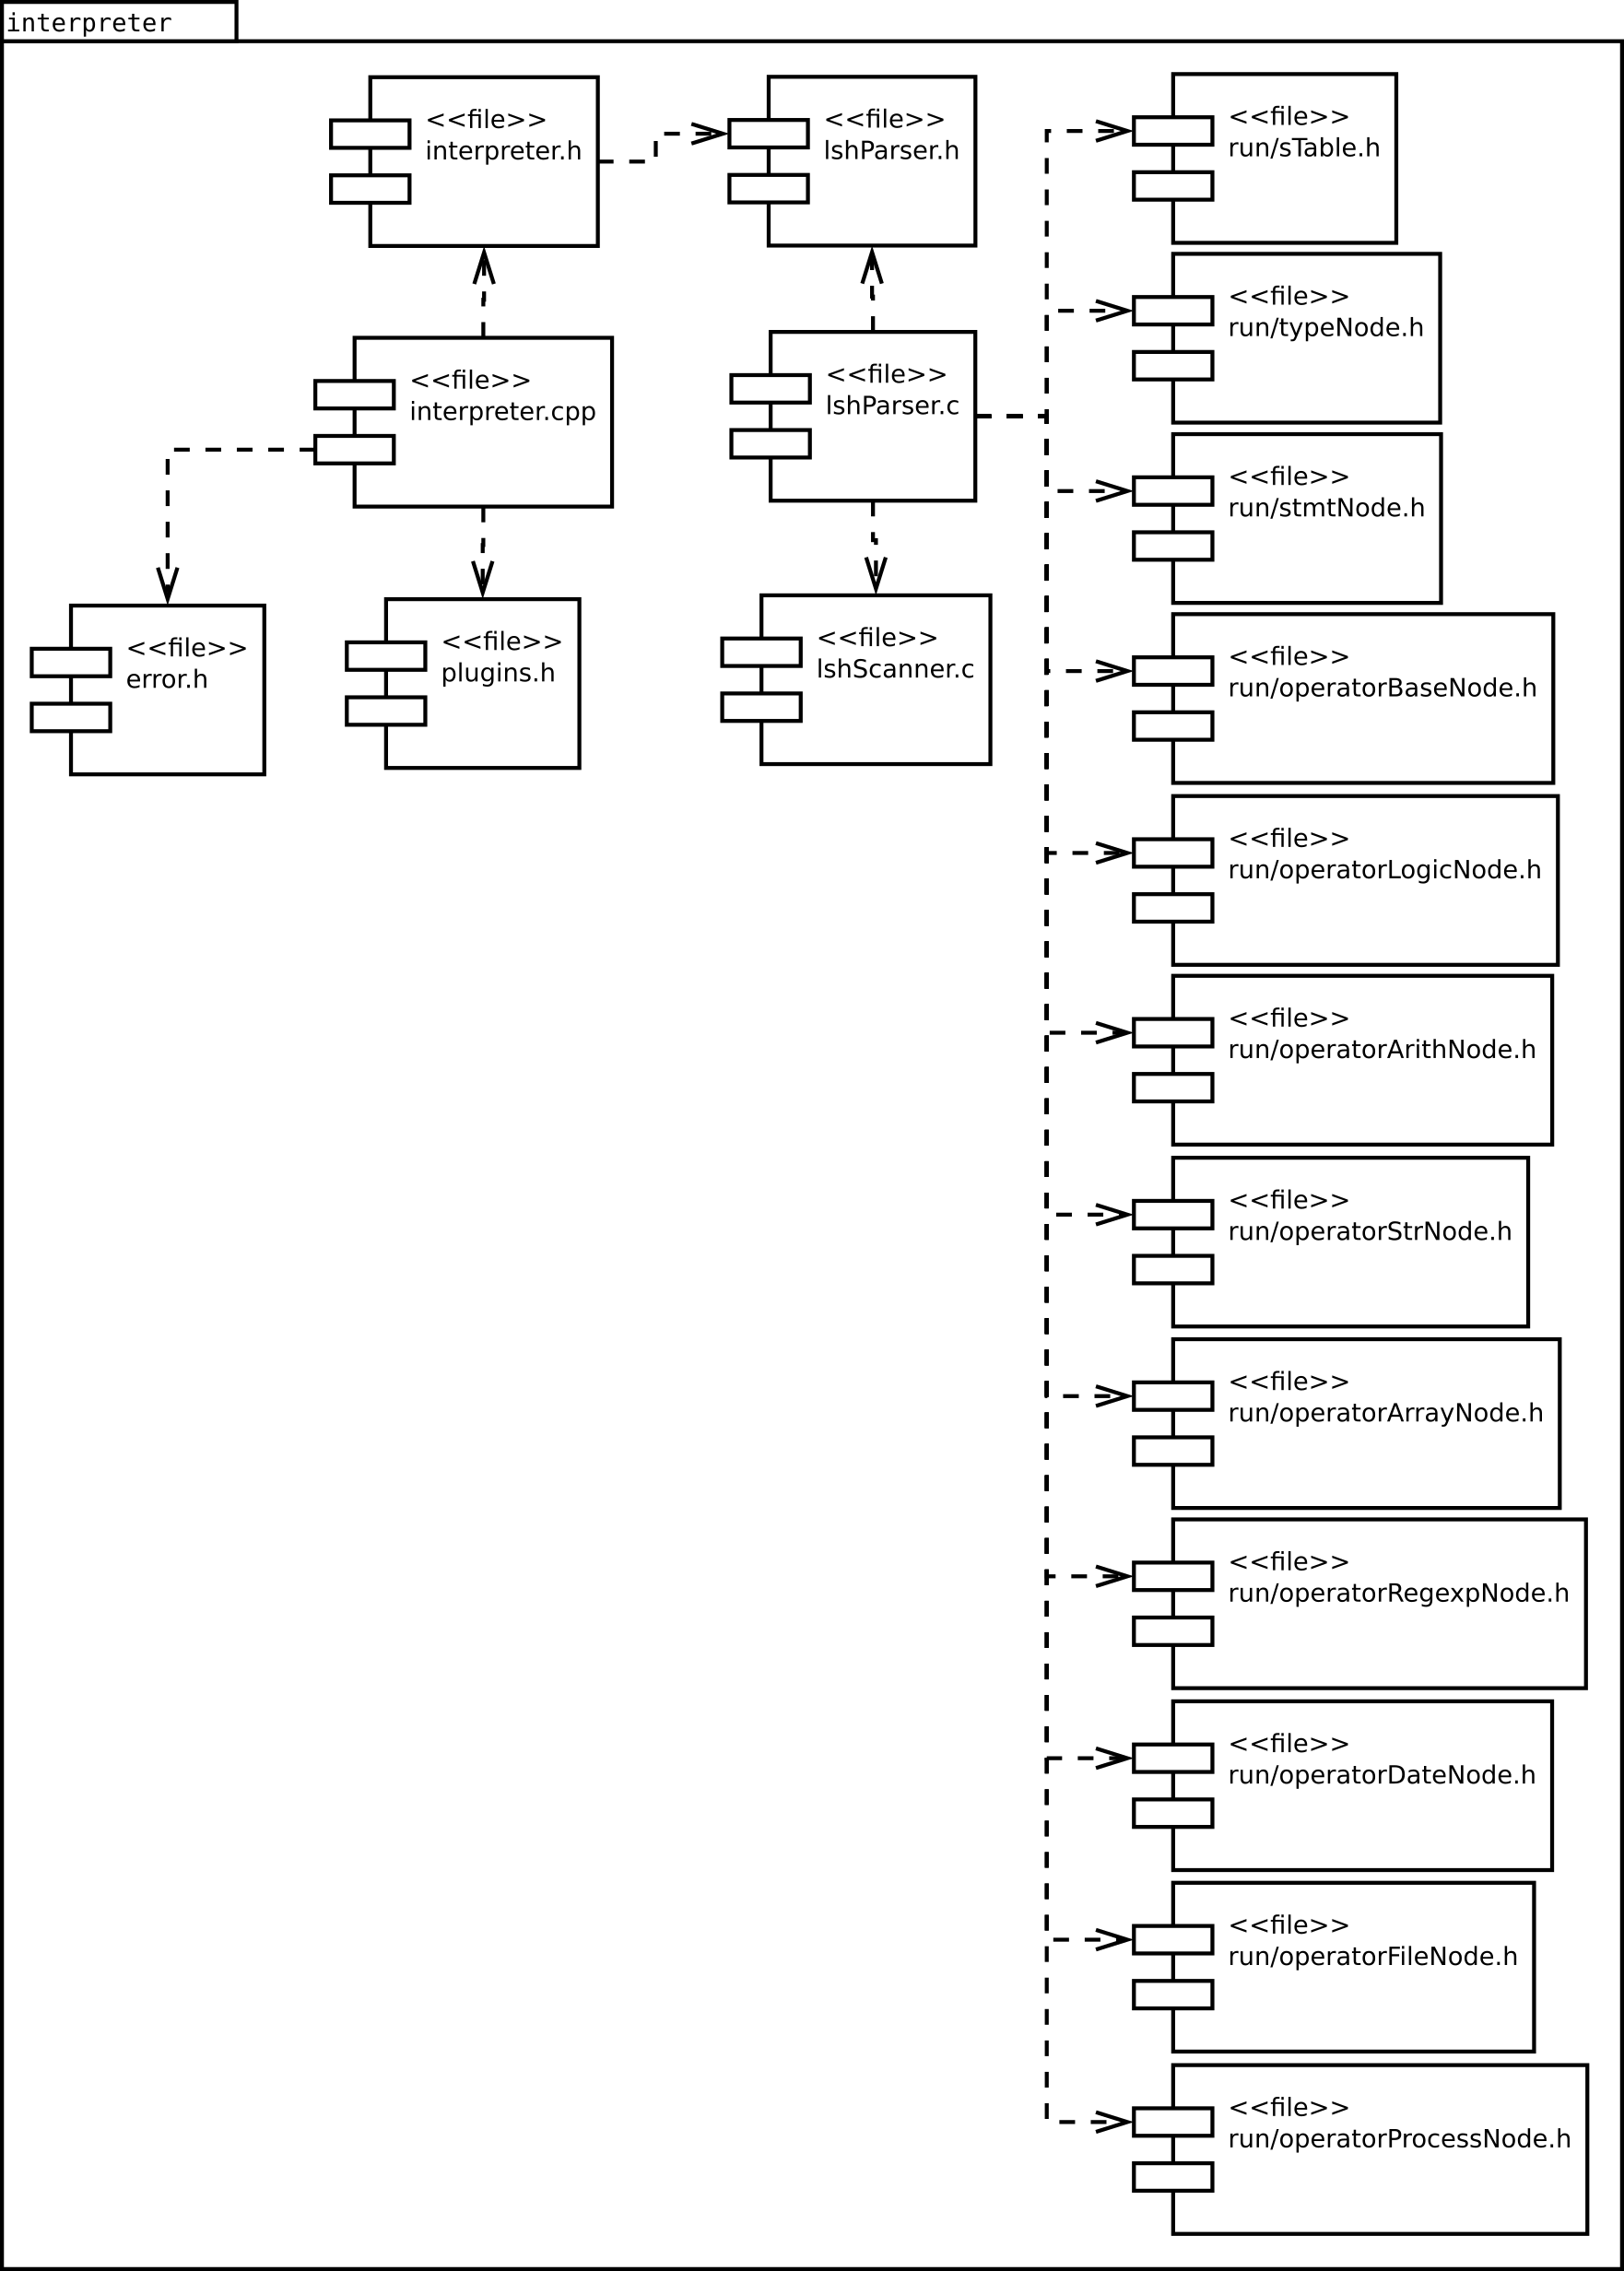
\includegraphics[scale=0.3]{files_arquitecture/interpreter.png} \\
\end{center}
\pagebreak
\begin{multicols}{2}
\begin{center}
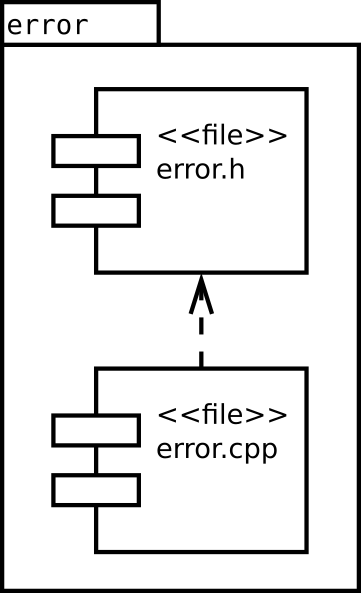
\includegraphics[scale=0.3]{files_arquitecture/error.png} \\
\end{center}
\begin{center}
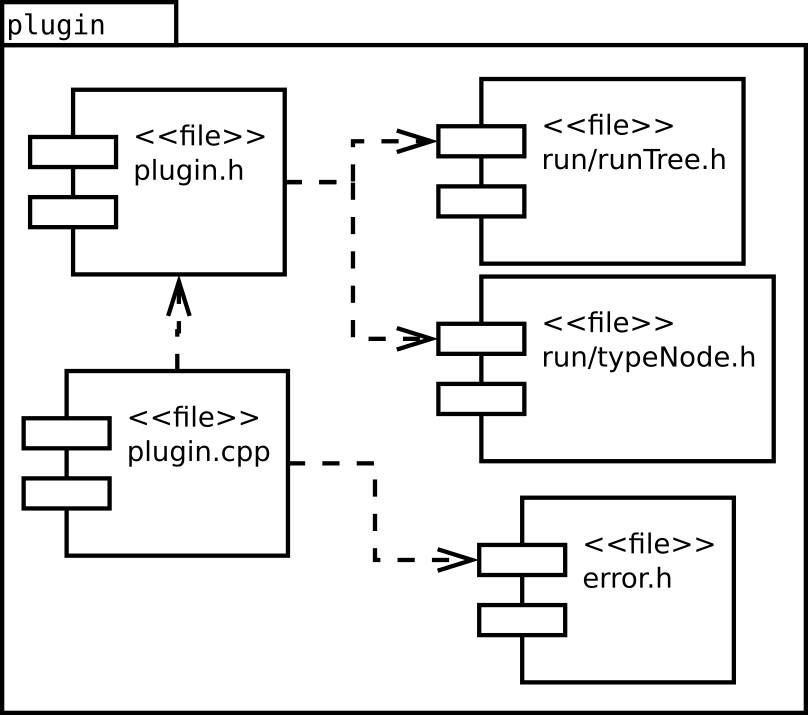
\includegraphics[scale=0.3]{files_arquitecture/plugin.png} \\
\end{center}
\end{multicols}

\begin{multicols}{2}
\begin{center}
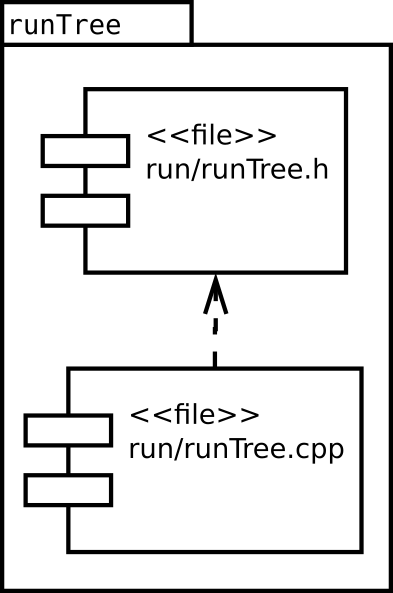
\includegraphics[scale=0.3]{files_arquitecture/runTree.png} \\
\end{center}
\begin{center}
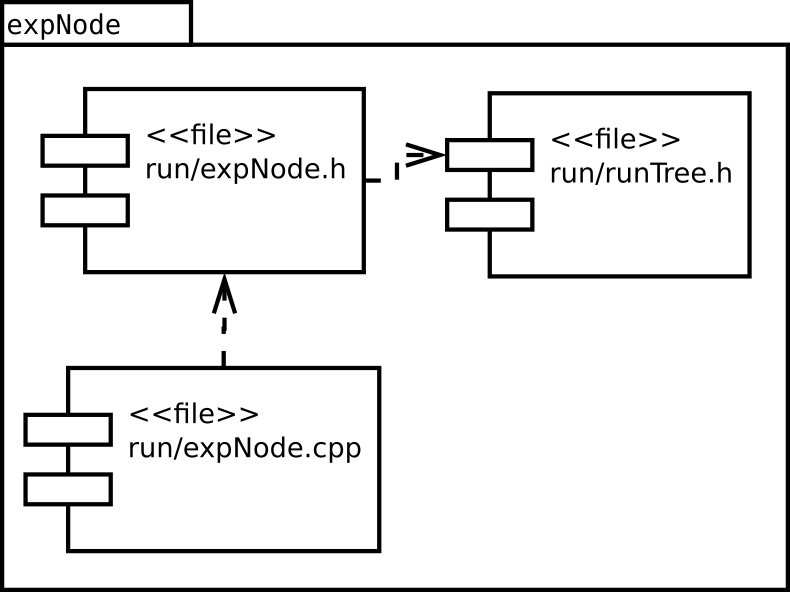
\includegraphics[scale=0.3]{files_arquitecture/expNode.png} \\
\end{center}
\end{multicols}

\begin{multicols}{2}
\begin{center}
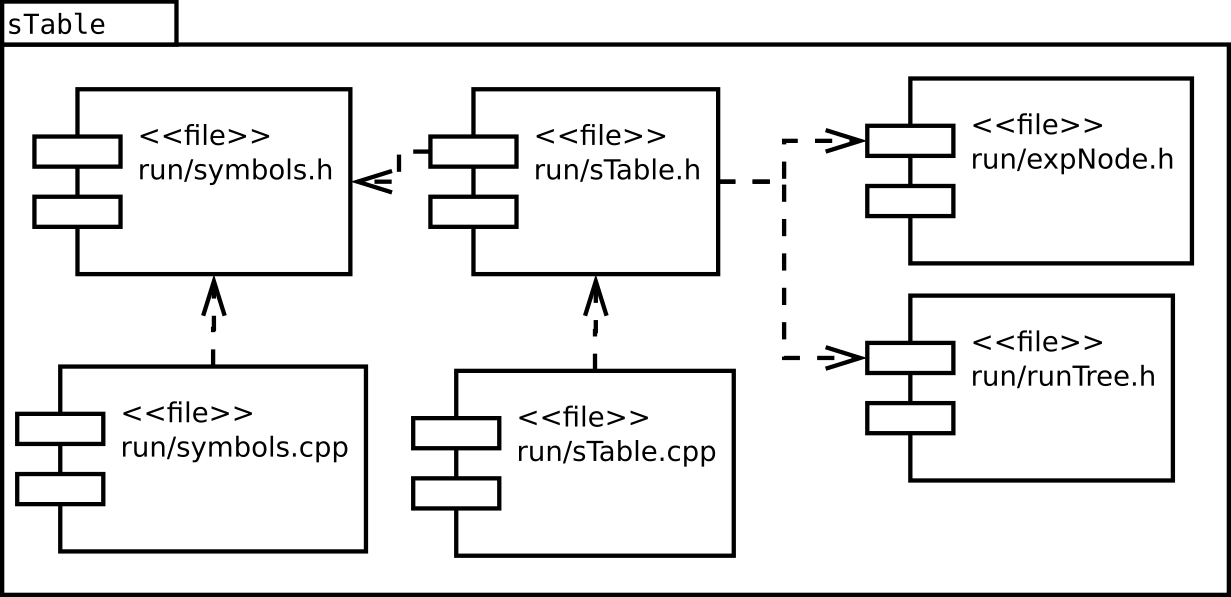
\includegraphics[scale=0.3]{files_arquitecture/sTable.png} \\
\end{center}
\begin{center}
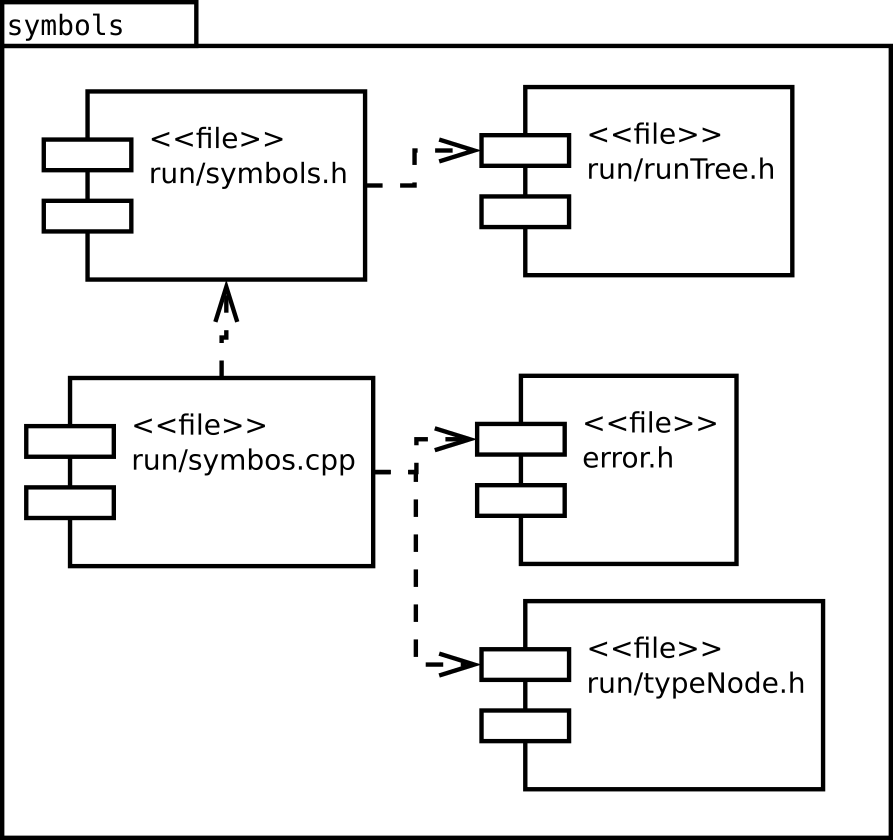
\includegraphics[scale=0.3]{files_arquitecture/symbols.png} \\
\end{center}
\end{multicols}

\begin{multicols}{2}
\begin{center}
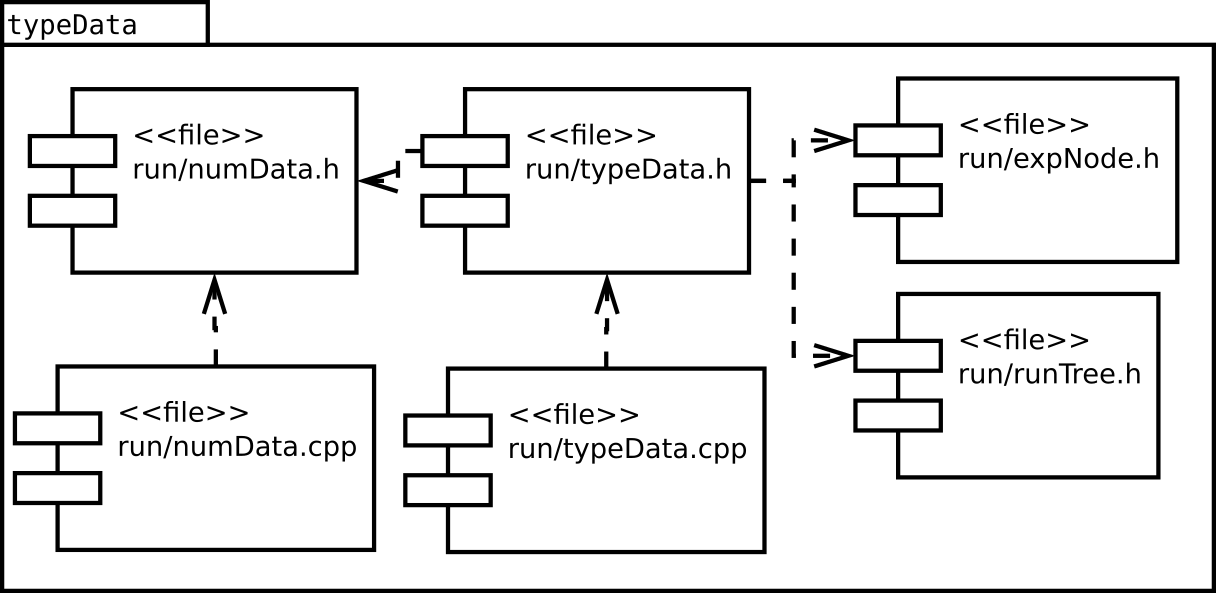
\includegraphics[scale=0.3]{files_arquitecture/typeData.png} \\
\end{center}
\begin{center}
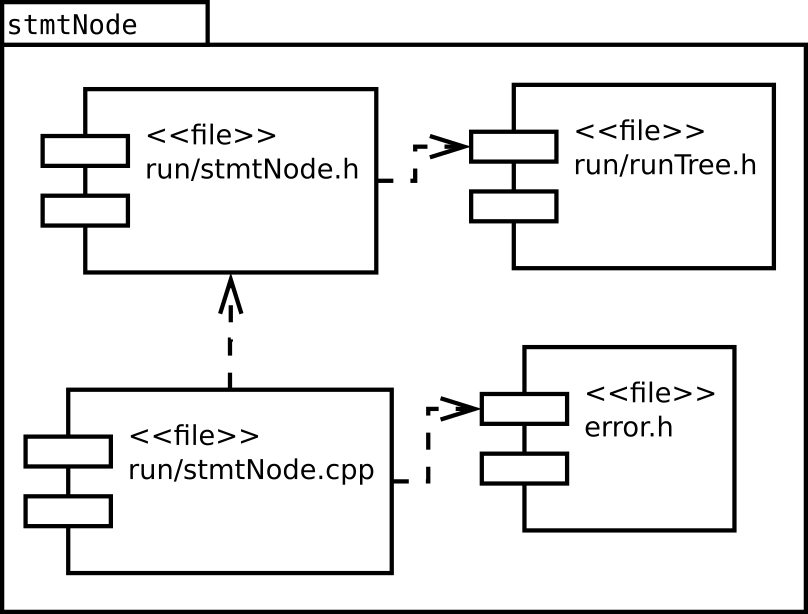
\includegraphics[scale=0.3]{files_arquitecture/stmtNode.png} \\
\end{center}
\end{multicols}
\pagebreak
\begin{multicols}{2}
\begin{center}
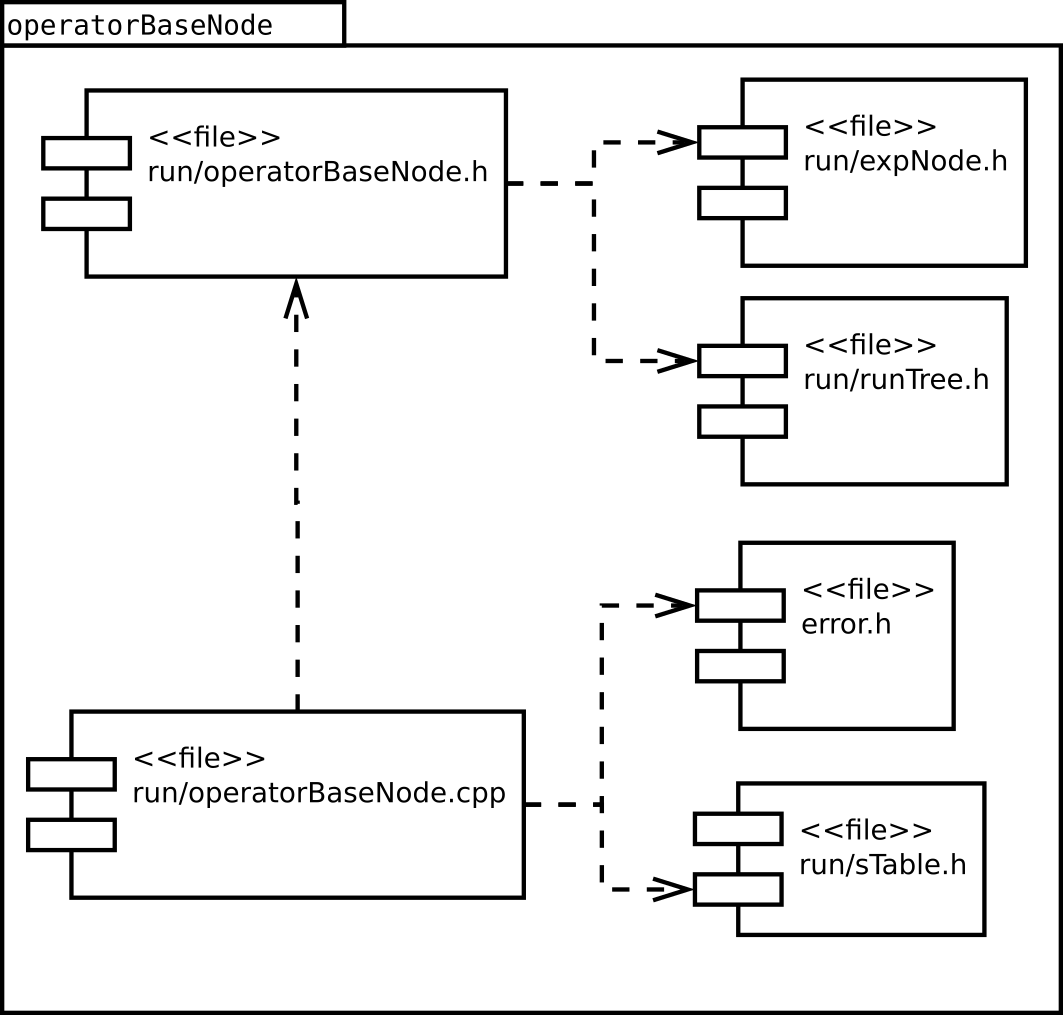
\includegraphics[scale=0.3]{files_arquitecture/operatorBaseNode.png} \\
\end{center}
\begin{center}
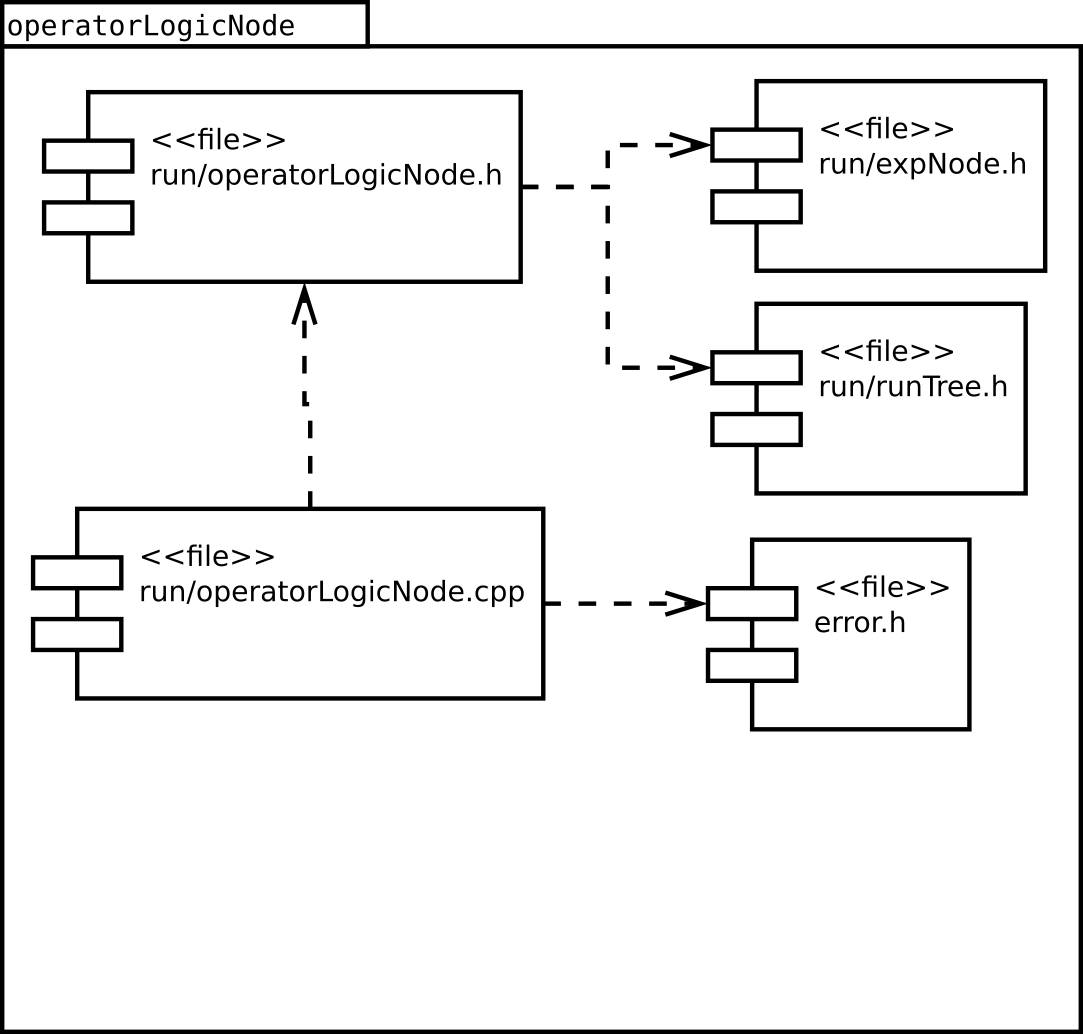
\includegraphics[scale=0.3]{files_arquitecture/operatorLogicNode.png} \\
\end{center}
\end{multicols}

\begin{multicols}{2}
\begin{center}
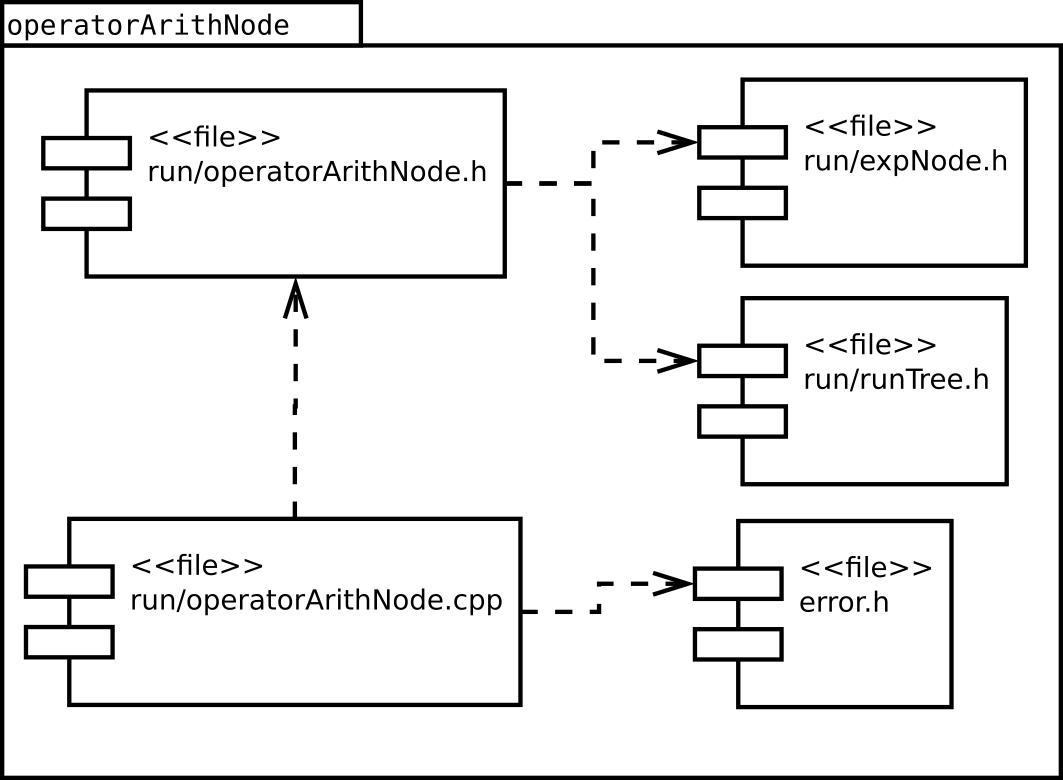
\includegraphics[scale=0.3]{files_arquitecture/operatorArithNode.png} \\
\end{center}
\begin{center}
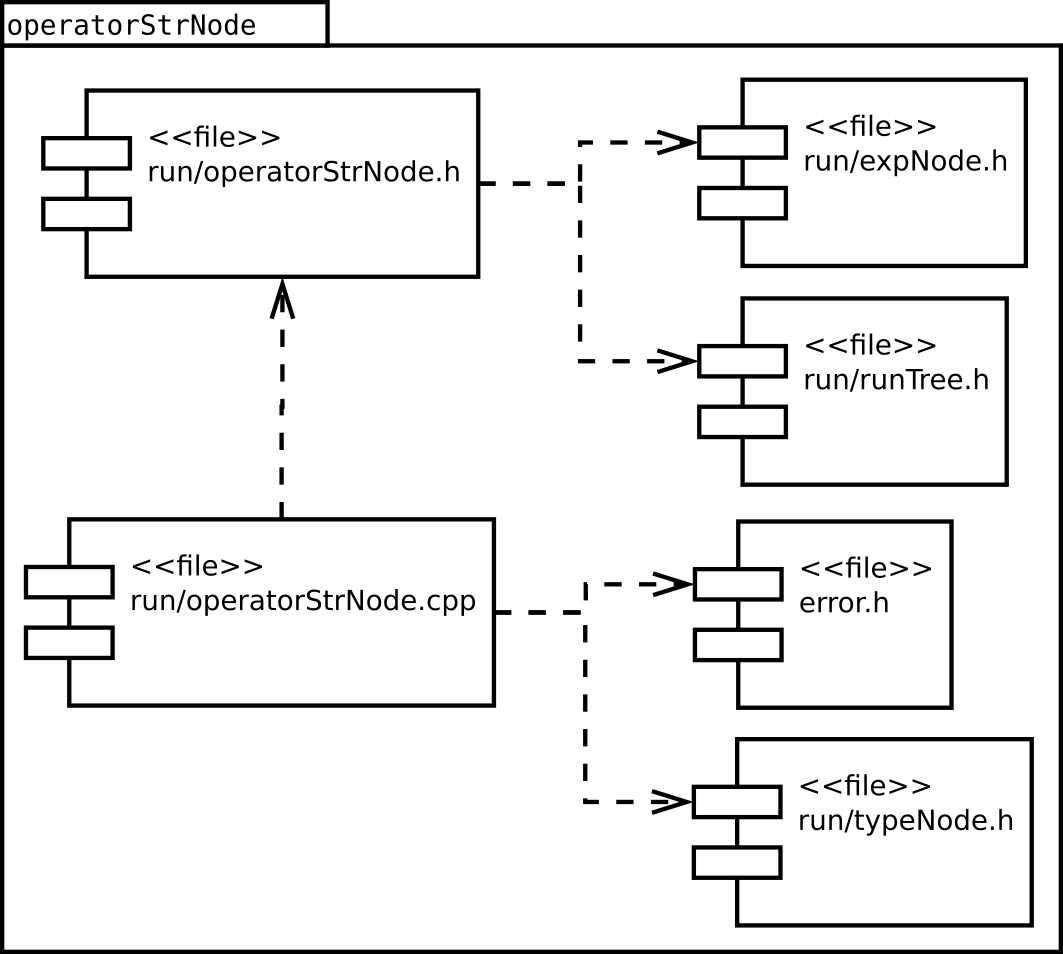
\includegraphics[scale=0.3]{files_arquitecture/operatorStrNode.png} \\
\end{center}
\end{multicols}


\begin{multicols}{2}
\begin{center}
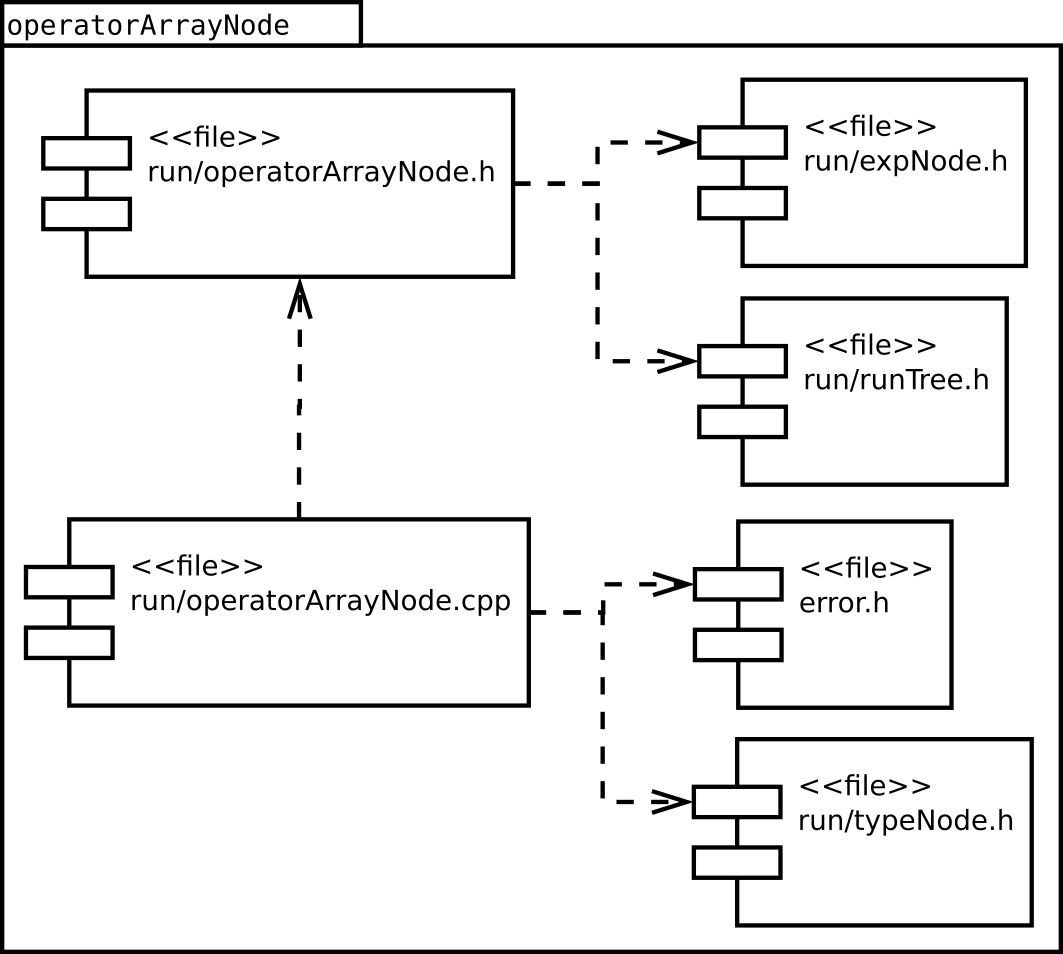
\includegraphics[scale=0.3]{files_arquitecture/operatorArrayNode.png} \\
\end{center}
\begin{center}
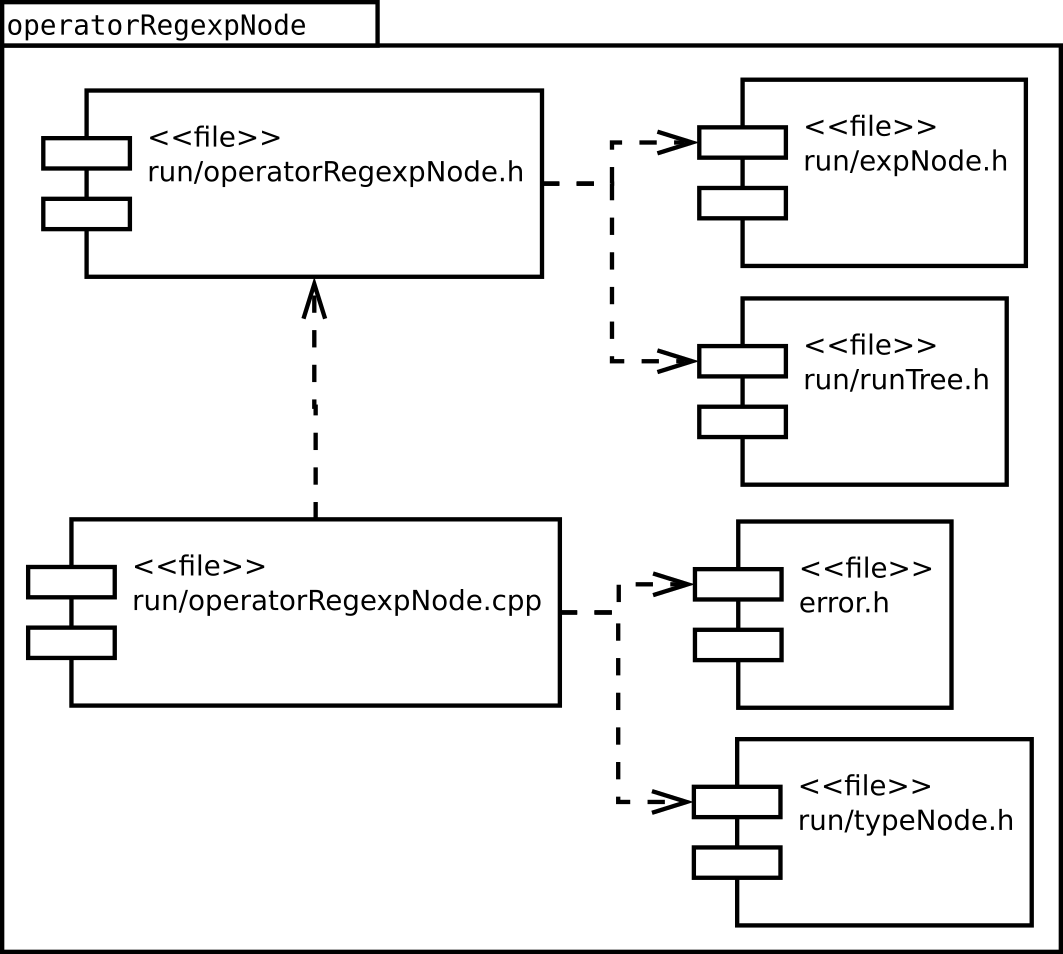
\includegraphics[scale=0.3]{files_arquitecture/operatorRegexpNode.png} \\
\end{center}
\end{multicols}

\begin{multicols}{2}
\begin{center}
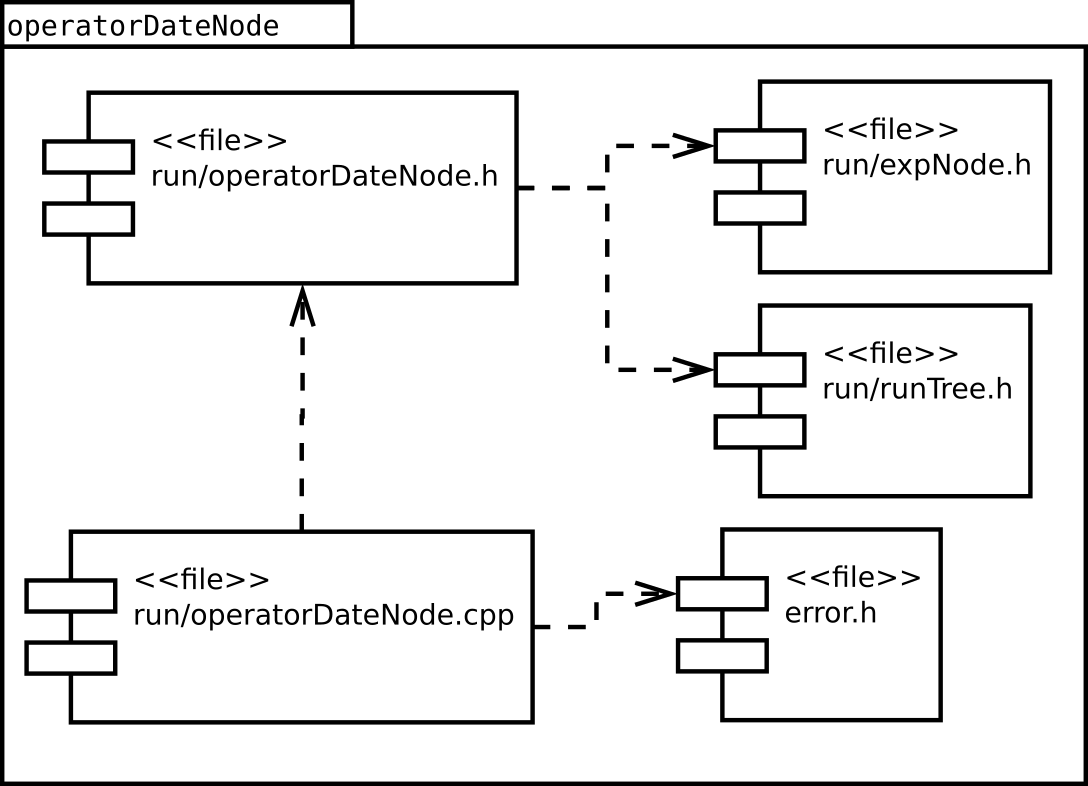
\includegraphics[scale=0.3]{files_arquitecture/operatorDateNode.png} \\
\end{center}
\begin{center}
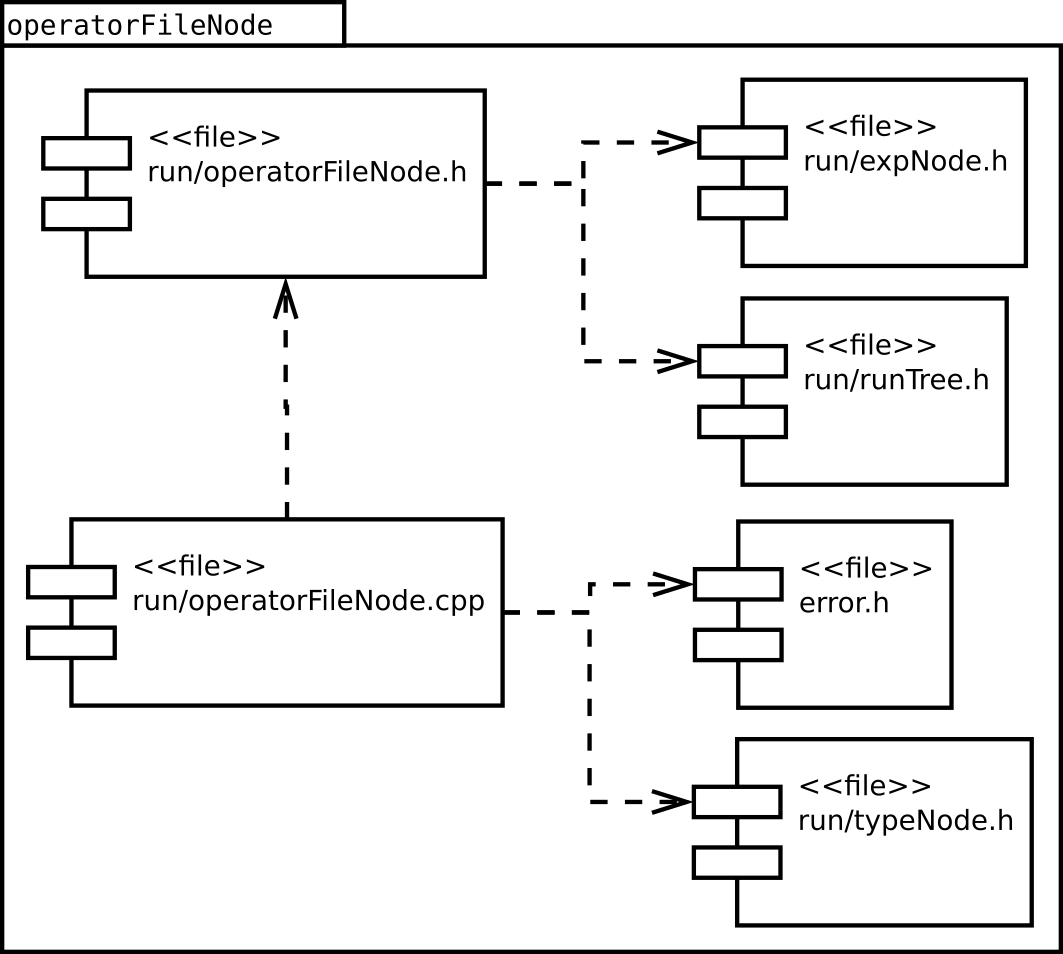
\includegraphics[scale=0.3]{files_arquitecture/operatorFileNode.png} \\
\end{center}
\end{multicols}


%~ \begin{multicols}{2}
\begin{center}
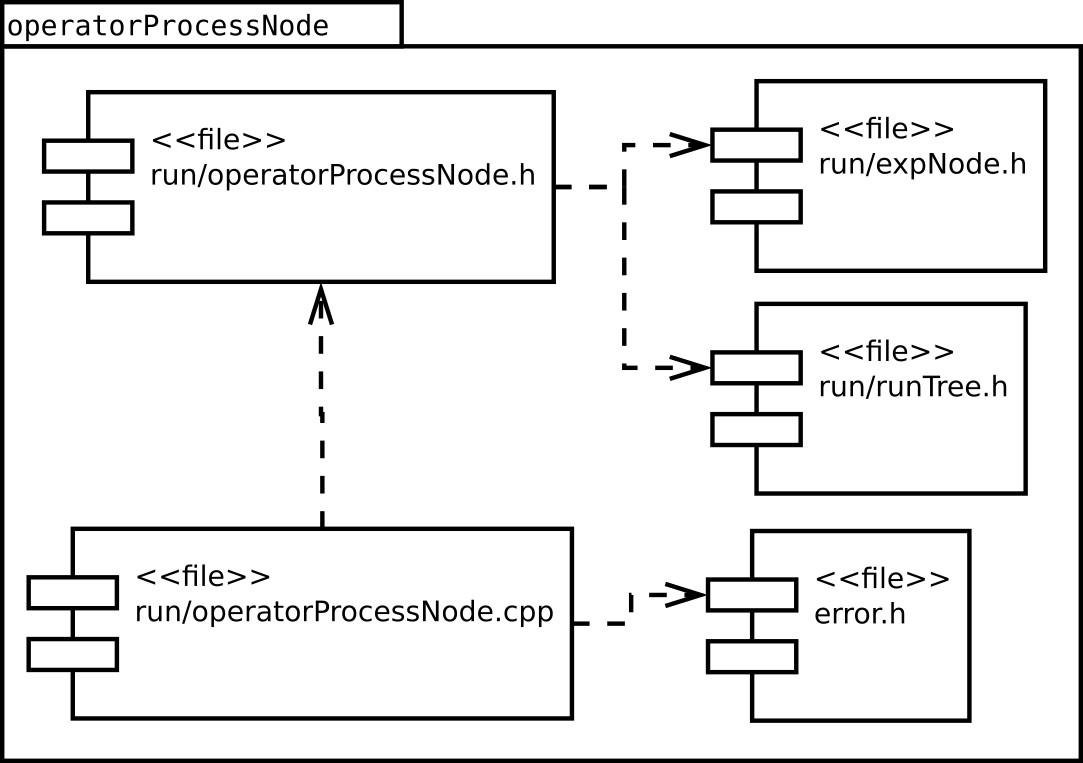
\includegraphics[scale=0.3]{files_arquitecture/operatorProcessNode.png} \\
\end{center}
%~ \end{multicols}

\section{Extractos de código fuente}
\subsection{Acceso a variable}

%~ \begin{lstlisting}[language=cpp]
\begin{myverbatim}
void idNode::run (bool resolvkey) {
   #if JSON==1
      interpreter::to_jsonRun(this);
   #endif
   sTable *table_ = sTable::sTable_use;
   refNode *str = new refNode(id_);
   exist_ = table_->exist (str);
   ref_ = table_->access (str);
   delete str;
   runNode *val = ref_->getRef();
   refNode * key = NULL;
   ref_ = refNode::resolved (val);
   if (privateNode::is)
      table_->setPrivate(new refNode (id_));
   if (!ref_->isprivate_)
      ref_->isprivate_ = privateNode::is;
   #if JSON==1
         interpreter::to_jsonSetValue(this, val);
   #endif
}
\end{myverbatim}

\subsection{Asignación}
\begin{myverbatim}
void asigNode::run () {
   runNode *node_aux = node2_, *nodeR_ = NULL;
   #if JSON==1
      interpreter::to_jsonRun(this);
   #endif
   ref_ = NULL;
   nexpNode::resolvedRef (node_aux);
   #if JSON==1
      if (node2_ != node_aux)
         interpreter::to_jsonRun(this);
   #endif
   if (!(bool)dynamic_cast<functionNode*>(node_aux) && node2_ == node_aux) {
      node_aux->run();
      #if JSON==1
         interpreter::to_jsonRun(this);
      #endif
   }
   nodeR_ = this->isRefNode (node_aux)?node_aux:expNode::clone (node_aux);
   noderef(nodeR_);
   #if JSON==1
      interpreter::to_jsonSetValue(this, nodeR_);
   #endif
   setValue (nodeR_);
}
\end{myverbatim}

\subsection{Operación suma}
%~ \begin{lstlisting}[language=cpp]
\begin{myverbatim}
void addNode::run () {
   #if JSON==1
      interpreter::to_jsonRun(this);
   #endif         
   runNode* op1 = node1_;
   runNode* op2 = node2_;
   nexpNode::resolved (op1);
   #if JSON==1
      interpreter::to_jsonRun(this);
   #endif      
   nexpNode::resolved (op2);
   #if JSON==1
      interpreter::to_jsonRun(this);
   #endif         
   numvalue_ = addNode::do_add (op1, op2);
   #if JSON==1
      interpreter::to_jsonSetValue(this, numvalue_);
   #endif
}
\end{myverbatim}

\end{document}
%%%%%%%%%%%%%%%%%%%%%%%%%%%%%%%%%%%%%%%%%%%%%%%%%%%%%%%%%%%%%%%%%%%%%%%%
%Fco. Javier Bohórquez Ogalla
